\chapter{EVALUATION}
This chapter presents the process of evaluating the effectiveness of the whole system and its features. At the same time, self-assessment of the work done by the group, from which the development direction of the topic
\section{Social media website}
\subsection{Evaluation metric}
\subsubsection{Website Grader powered by HubSpot}
This tool evaluate a website based on 4 criteria: performance, mobile, SEO, security.\\
\textbf{Overall}\\
The social media website is scored:
\begin{itemize}
\item Performance: 22/30
\item Mobile: 30/30
\item SEO: 10/30
\item Security: 10/10
\end{itemize}
Compared to \textit{9gag} which is a well known social media for entertainment. 
\begin{table}[H]
\begin{tabular}{|l|c|l|}
\hline
            & \multicolumn{1}{l|}{The social media website} & 9gag  \\ \hline
Performance & 22/30                                         & 24/30 \\ \hline
Mobile      & 30/30                                         & 30/30 \\ \hline
SEO         & 10/30                                         & 30/30 \\ \hline
Security    & 10/10                                         & 10/10 \\ \hline
\end{tabular}
\end{table}
This result is acceptable because 9gag has grown and improved for a lengthy duration since it first launched in 2008. In contrast, the social media website has just been developed for a short amount of time.\\
\textbf{Performance}\\
\begin{itemize}
\item Page size: The heavier the site page, the slower the load.
\item Page request: The more HTTP requests your website makes, the slower it becomes.
\item Page speed: Load time
\item Browser caching: Browser caching speeds up your website by storing frequently used content in local memory.
\item Page redirect: Page redirects add an additional loading cycle, increasing the time to display the page.
\item Compression: When your JavaScript and CSS are properly compressed, it makes your website run much faster.
\item Render blocking: Remove or defer JavaScript and CSS that interferes with loading above-the-fold content.
\begin{table}[H]
\begin{tabular}{|c|c|c|}
\hline
                & The social media website & 9gag              \\ \hline
Page size       & 715 KB                   & 337 KB            \\ \hline
Page requests   & 34                       & 74                \\ \hline
Page speed      & 0.4                      & 0.5               \\ \hline
Browser caching & \checkmark               & \checkmark        \\ \hline
Page redirects  & No page redirects        & No page redirects \\ \hline
Compression     & $\times$                 & \checkmark        \\ \hline
Render blocking & $\times$                 & $\times$            \\ \hline
\end{tabular}
\end{table}
\end{itemize}
\textbf{Mobile}\\
Responsive design gives the social media the ability to scale on different device types which also enable mobile friendliness.\\
\textbf{SEO}\\
\begin{itemize}
\item Page title: Page titles should be no longer than 70 characters in length and not repeat keywords.
\item Meta description: Meta descriptions should be no longer than 300 characters in length and should be relevant to the page.
\item Headings: Heading tags distinguish headings from core page content.
\item Sitemap: Site maps help users navigate your site quickly and easily.
\end{itemize}
\begin{table}[H]
\begin{tabular}{|c|c|c|}
\hline
                 & The social media website & 9gag \\ \hline
Page titles      & \checkmark               & \checkmark  \\ \hline
Meta description & $\times$                 & \checkmark  \\ \hline
Headings         & $\times$                 & \checkmark  \\ \hline
Sitemap          & $\times$                 & \checkmark  \\ \hline
\end{tabular}
\end{table}
In this project, marketing is not focused on, this result is inevitable.
\textbf{Security}\\
SSL certificates protect the social media website from attacks and give visitors confidence that your site is authentic and trustworthy.

\subsubsection{GTmetrix developed by GT.net}
In this section, the used evaluation metric is GTmetrix, a tool for Webpage Performance Analysis. GTmetrix is a combination of two favorite analyze tools: Google PageSpeed and Yahoo! YSlow. It also provides other website’s related data: Page Load Time, Total Page Size and Total Number of Requests. Result data will be visualized for better evaluation.

\begin{itemize}
\item Total Page Size: also called Page Weight, is the overall size of a Webpage. It includes the size of all files that created that Webpage: HTML document, images, stylesheet,…
\item Page Load Time: indicates the time for a webpage and all its components loaded.
\item Total Number of Requests: is the total number of request the webpage has been made.
\item PageSpeed Score and YSlow Score: Score of the webpage based on Google PageSpeed and Yahoo! YSlow criteria.
\end{itemize}

The following image is the Performance Report for this social media website (which is hosted on \href{https://god-eye-cc14.herokuapp.com/}{https://god-eye-cc14.herokuapp.com/}).

\begin{center}
    \begin{figure}[H]
    \centering
    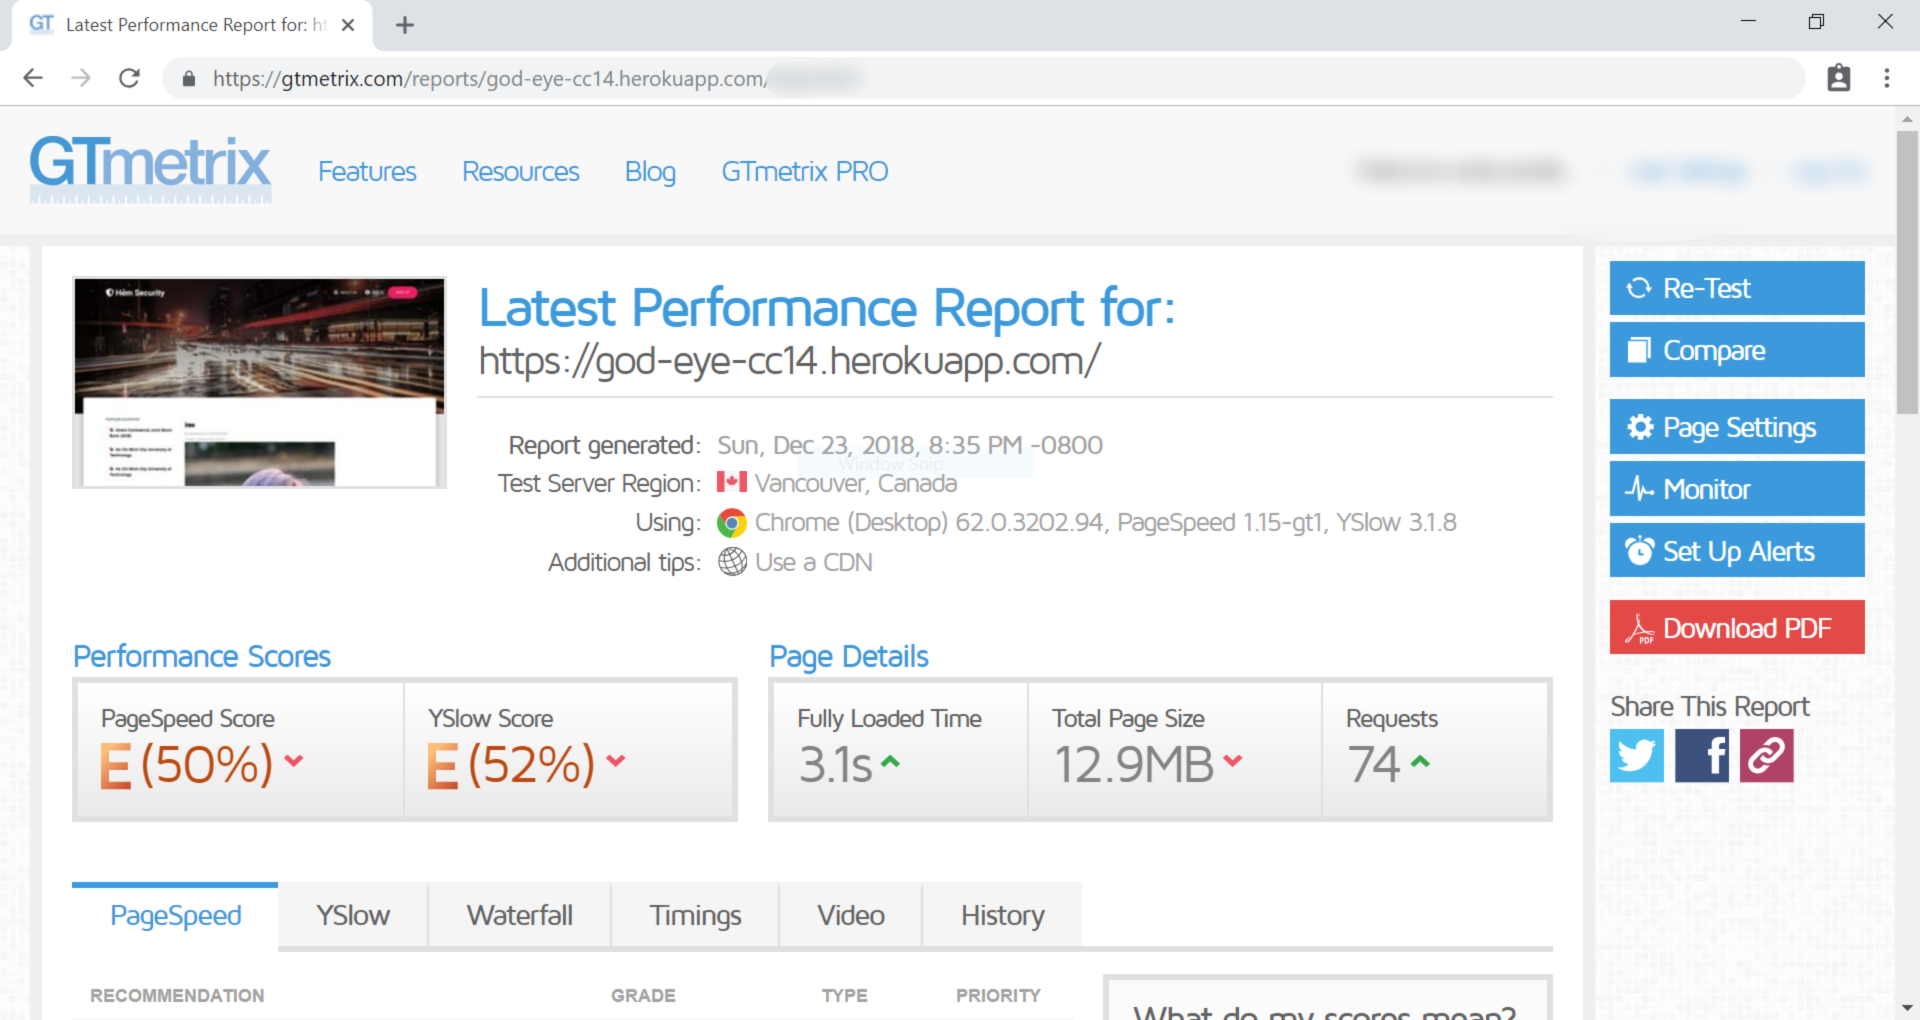
\includegraphics[width=1\columnwidth]{images/chap5/gtmetrix-result.PNG}
    \caption{The Social Media Website's Performance Report from GTmetrix}
    \end{figure}
\end{center}

The performance of this Social Media Website is compared with 9GAG (\href{https://9gag.com}{https://9gag.com}) and Facebook  Vietnam (\href{https://facebook.com/FacebookVietnam}{https://facebook.com/FacebookVietnam}).

\begin{center}
    \begin{figure}[H]
    \centering
    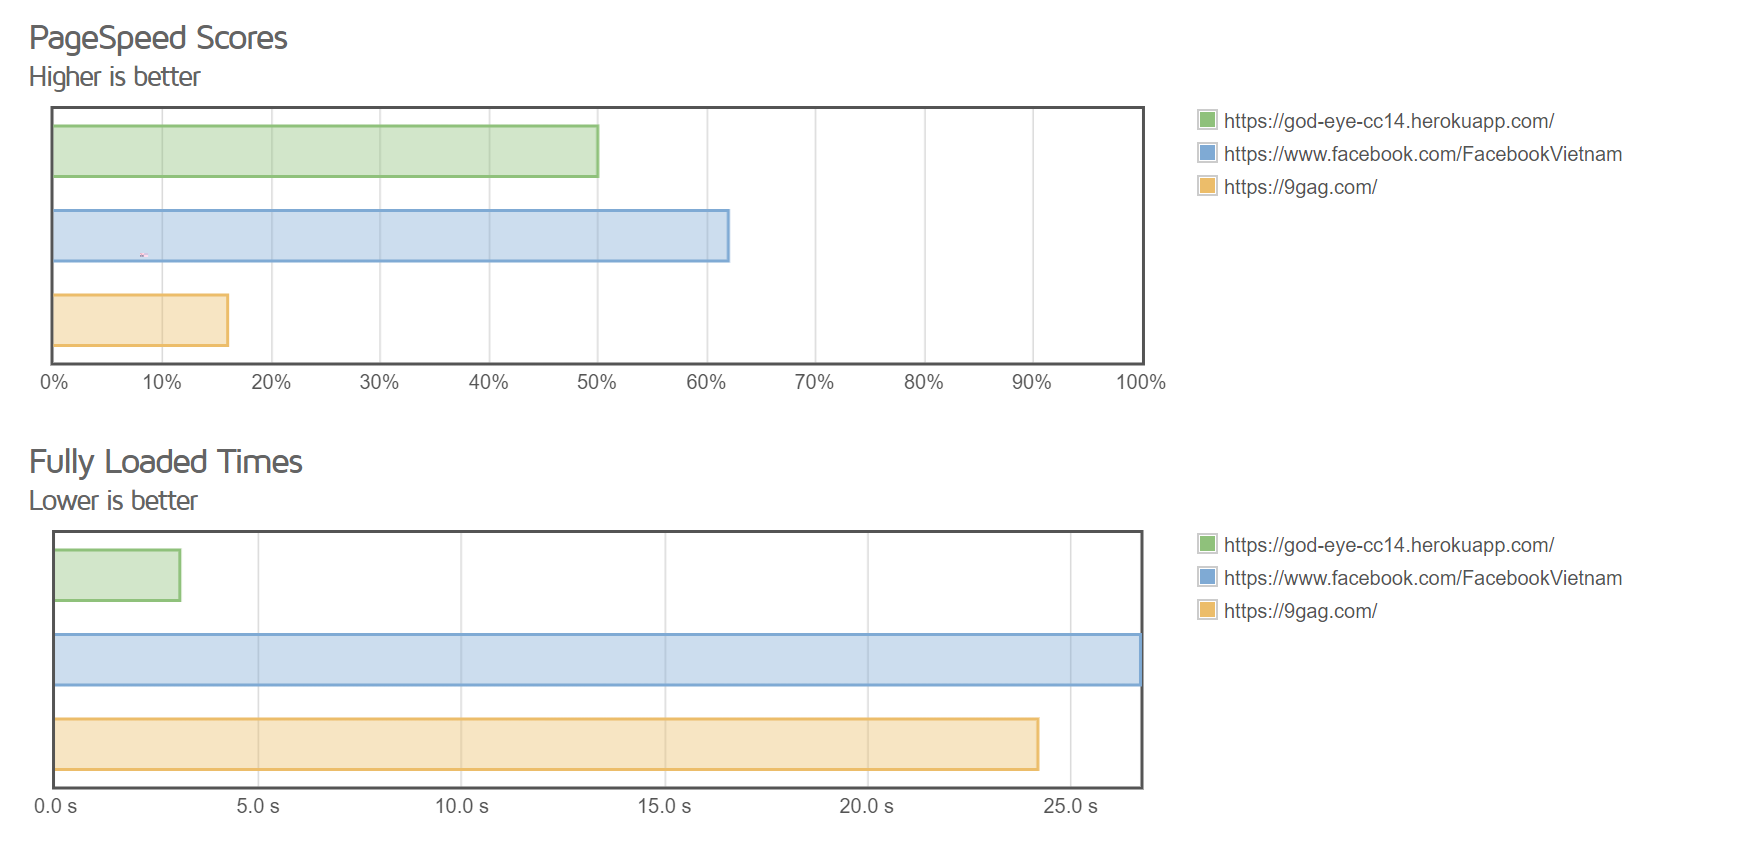
\includegraphics[width=1\columnwidth]{images/chap5/gtmetrix-graph-1.PNG}
    \caption{The Social Media Website's Performance compared with 9GAG and Facebook (1)}
    \end{figure}
\end{center}

\begin{center}
    \begin{figure}[H]
    \centering
    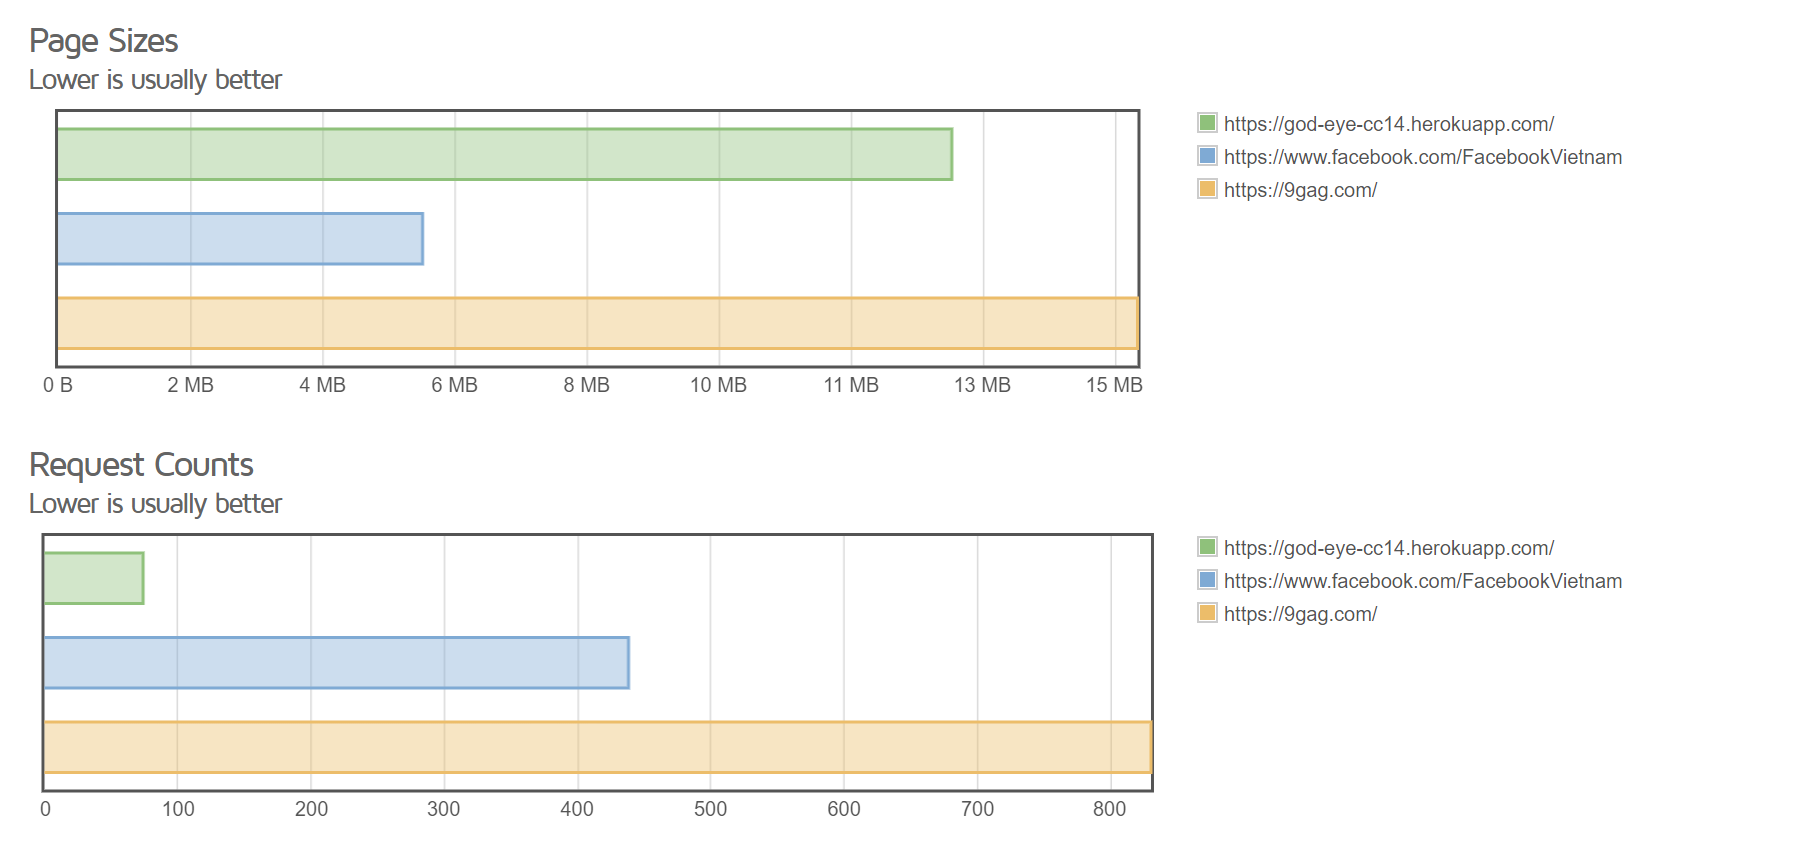
\includegraphics[width=1\columnwidth]{images/chap5/gtmetrix-graph-2.PNG}
    \caption{The Social Media Website's Performance compared with 9GAG and Facebook (2)}
    \end{figure}
\end{center}

In some criteria like Request Counts and Fully Loaded Time, the Social Media website has advantages over 9GAG and Facebook Vietnam. Other criteria (PageSpeed Score and Page Sizes) can be enhanced in further improvement.

\subsubsection{PageSpeed Insights}
The system is evaluated by PageSpeed which is a highly authentic tool of one of the best IT company recently which is Google. There are many estimation criteria such as lab data, opportunities, performance, passed audits. 

The website uses the simulation runtime settings and slow 4G internet connection with information as below:
\begin{itemize}
	\item URL: \href{http://god-eye-cc14.herokuapp.com/}{https://god-eye-cc14.herokuapp.com/}
	\item Fetch time: Dec 24, 2018,  11:54:20 AM GMT+7
	\item Device: Emulated Nexus 5X
	\item Network throttling: 150 ms TCP RTT, 1,638.4 Kbps throughput (Simulated)
	\item CPU throttling: 4x slowdown (Simulated)
	\item User agent (host): Mozilla/5.0 (Windows NT 10.0; Win64; x64) AppleWebKit/537.36 (KHTML, like Gecko) Chrome/70.0.3538.110 Safari/537.36
	\item User agent (network): Mozilla/5.0 (Linux; Android 6.0.1; Nexus 5 Build/MRA58N) AppleWebKit/537.36 (KHTML, like Gecko) Chrome/71.0.3559.0 Mobile Safari/537.36
	\item CPU/Memory Power: 472
\end{itemize}
\begin{center}
	\begin{figure}[H]
		\centering
		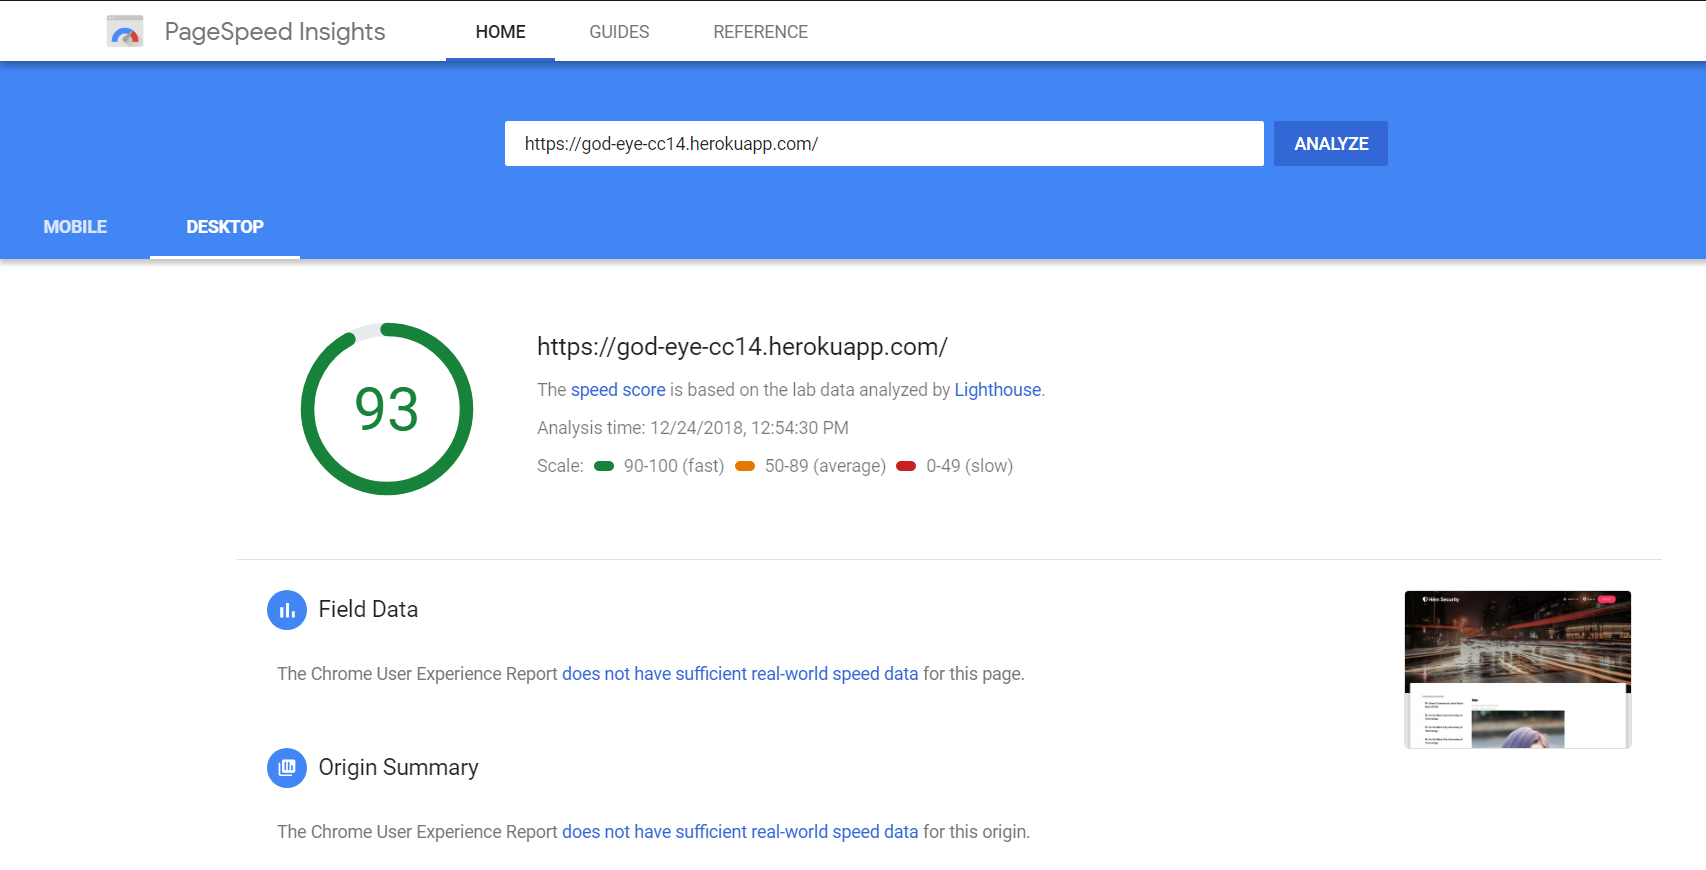
\includegraphics[width=1\columnwidth]{images/chap5/pagespeed1.PNG}
		\caption{PageSpeed evaluate performance website}
	\end{figure}
\end{center}
\begin{center}
	\begin{figure}[H]
		\centering
		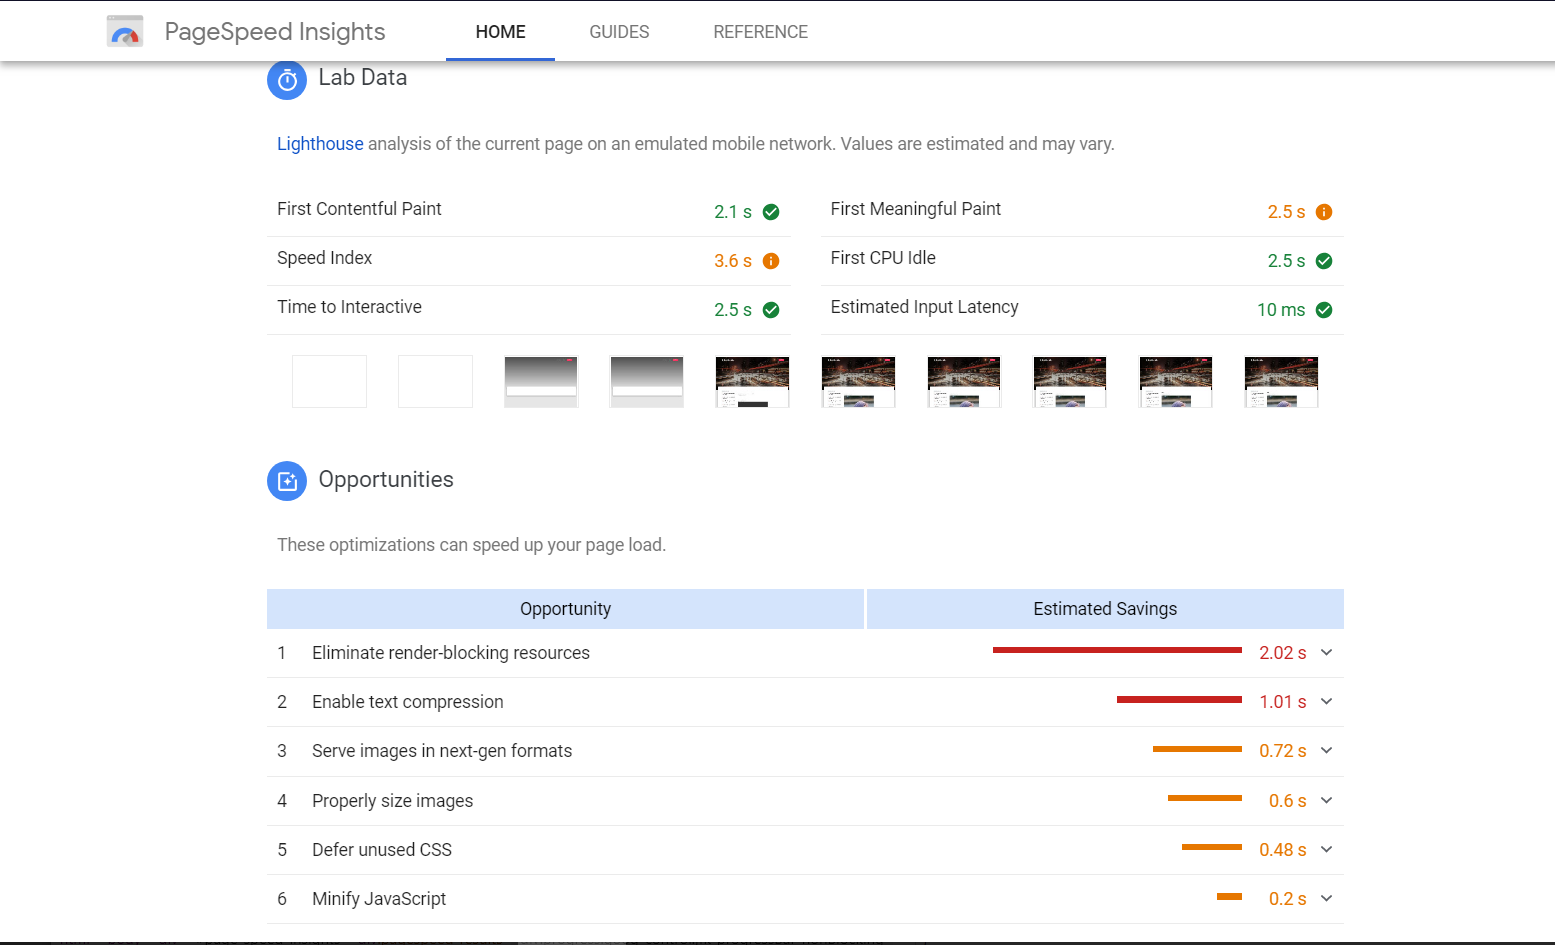
\includegraphics[width=1\columnwidth]{images/chap5/pagespeed2.PNG}
		\caption{PageSpeed evaluate lab data and opportunities}
	\end{figure}
\end{center}
\begin{center}
	\begin{figure}[H]
		\centering
		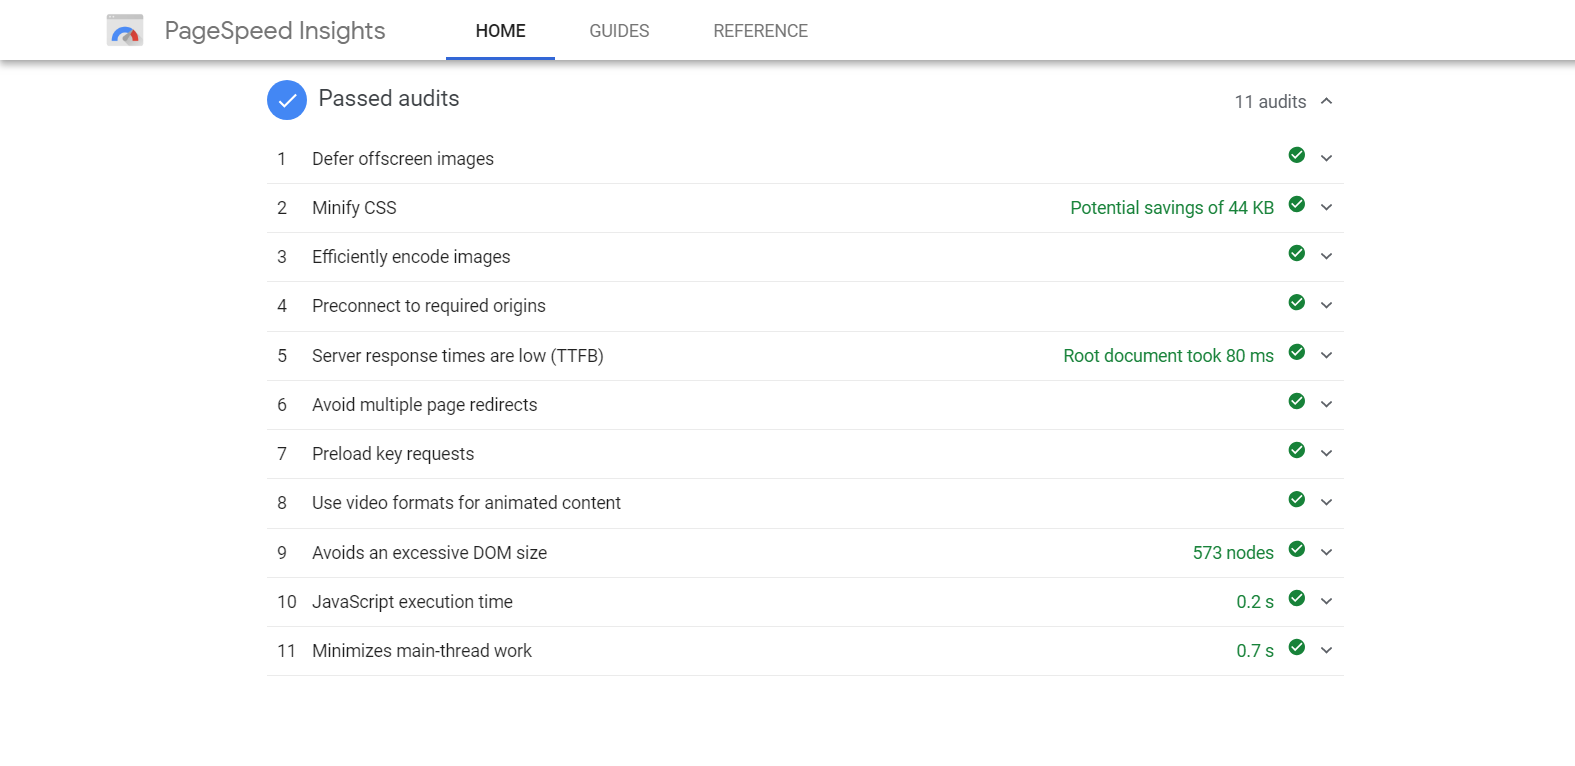
\includegraphics[width=1\columnwidth]{images/chap5/pagespeed3.PNG}
		\caption{PageSpeed evaluate passed audits}
	\end{figure}
\end{center}
 Therefore, the tool has evaluated its effectiveness; even it is run with 4G slow internet , it can fully operate the above criteria
\subsection{Result}
